\chapter{Randomized Algorithms in Numerical Linear Algebra}

%------------------------------------------------------------------------------------------------------
\section{Least Squares Problems}
Consider the linear system
\begin{equation}\label{AXB}
A x =b ,
\end{equation}
where $A \in \mathbb{R}^{m \times n}, b \in \mathbb{R}^{m}, m \gg n, $  and $rank(A) = n$.
System (\ref{AXB}) has the least squares solution
\begin{equation}\label{OPT}
x_{opt} = argmin_{x} \| Ax -b\|_2^2 .
\end{equation}
$x_{opt}$ is also the solution of the normal equation
\begin{equation}\label{NOR}
A^T A x = A^T b.
\end{equation}
Suppose $\bold{y} = (y_1,\cdots,y_n)'$  is the response or target variable.

$$\bold{X} = \begin{bmatrix} x_{11} ,&\cdots,& x_{1p}\\
                                                \cdots,&\cdots,&\cdots \\
                                                x_{n1},&\cdots,&x_{np} \end{bmatrix}
                 = (\bold{x_1},\cdots,\bold{x_p})$$
is the $n \times p$ data matrix of the $n$ observations on the $p$ variables.

The linear regression is to find the parameter $\bold{\beta}$ for a 'best' prediction of $\bold{y}$, which is to minimize the 2 norm of error
$$\| \bold{y} - \bold{X} \bold{\beta} \|_2^2.$$

The least squares estimator $\beta_{opt}$ is given by
$$
\beta_{opt} = (\bold{X}^T \bold{X})^{-1} \bold{X}^T \bold{y}.
$$
%-----------------------------------------------------------------------------------------------------------------
\section{Traditional Methods}
%------------------------------------------------


\subsection{QR Decomposition}

Compute
$$A = QR,$$
where $Q$ is an orthogonal matrix and $R$ is an upper triangular matrix.

 \begin{figure}[htbp]
    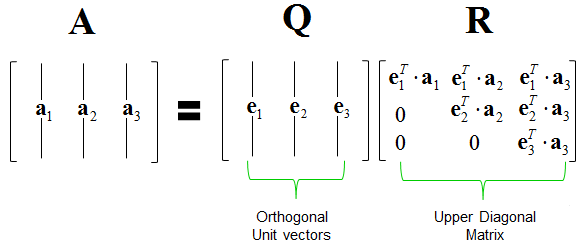
\includegraphics[width=1\textwidth]{qrd}
    \caption{QR Decomposition}
\end{figure}

Complexity of QR decomposition is {\color{red} $O(mn^2)$}.



%------------------------------------------------
\subsection{SVD Decomposition}

Compute
$$
A = U \Sigma V^T,
$$
where
\begin{itemize}
\item $U$ is a $m \times m $ orthogonal matrix \\
\item $\Sigma$ is a diagonal $m \times n$ matrix with non-negative real numbers on the diagonal and \\
\item $V$ is a $n \times n $ orthogonal matrix.
\end{itemize}
The diagonal entries are $\sigma_i$ of $\Sigma$ are known as the singular values of $A$. \\
 \begin{figure}[htbp]
    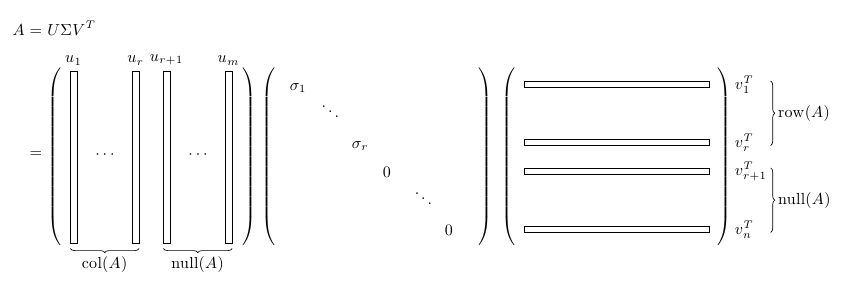
\includegraphics[width=1\textwidth]{svd2}
\end{figure}
Complexity of SVD decomposition is {\color{red} $O(mn^2)$}.


%------------------------------------------------



\subsection{Conjugate Gradient Method}

Apply the conjugate gradient method to the normal equation (\ref{NOR})
$$
A^T A x = A^T b.
$$
Complexity:
\begin{itemize}
\item The computation cost at each step is  $O(mn)$  for $A^T(Ax)$. \\
\item To achieve accuracy $\epsilon$, we need $ k = log_{\frac{\sqrt{\kappa(A^T A)} -1}{\sqrt{\kappa(A^T A)} +1}} \frac{\epsilon}{2} \approx 2 |log(\epsilon)|\kappa(A)$ steps. \\
\item The total complexity is
{\color{red}
$$
O(m n \kappa(A) |log(\epsilon)|).
$$
}
\end{itemize}

%------------------------------------------------

\subsection{Kaczmarz Method}


Denote the rows and columns of $A$ by $A^{(1)}, \cdots, A^{(m)}$ and $A_{(1)},\cdots,A_{(n)},$ respectively (both viewed as columns vectors). The Kaczmarz Scheme is given by
\begin{tcolorbox}
procedure $(A,b,T)$ \\
\quad Set\quad $ x^{(0)} $ \quad to by any vector in the row space of $A$\\
\quad for $k = 0,1,2,\cdots, T-1$ do \\
\quad \quad $ik \equiv k \Mod{m}$ \\
\quad \quad Set $x^{(k+1)} = \mathcal{P}_{A^{(ik)},b_{ik}}(x^{(k)}) $\\
\quad end for \\
\quad Output $x^{(T)}$  \\
end procedure
\end{tcolorbox}


\subsubsection{Orthogonal Projection}
We define the orthogonal projection of $\mathbf{x}$ onto the hyperplane by \quad $\mathbf{c}^T \mathbf{x} = d$:
$$
\mathcal{P}_{\mathbf{c},d}(\mathbf{x}) = \mathbf{x} - \frac{\mathbf{c}}{\| \mathbf{c} \|_2} (\mathbf{c} ^T \mathbf{x} - d).
$$
The operator does an orthogonal projection of the current estimate vector $\mathbf{x}$ onto the hyperplane $\mathbf{c}^T \mathbf{x} =d$.
\begin{figure}[htbp]
    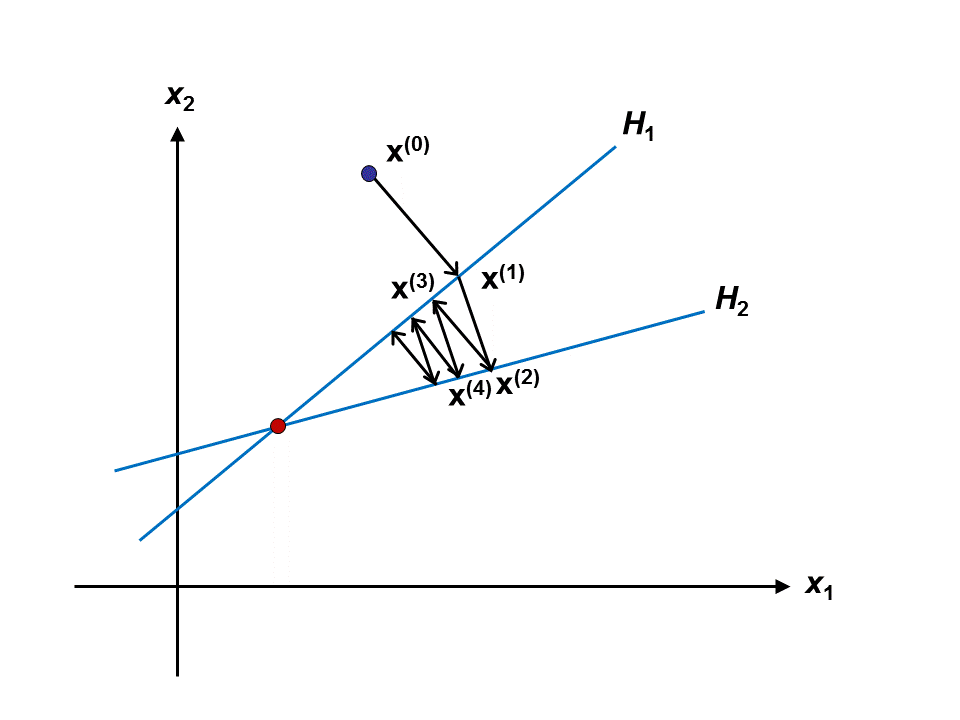
\includegraphics[width=\textwidth]{kaczmarz-method1.png}
    \caption{Kaczmarz Method}
    \label{fig:kaczmarz method}
\end{figure}

\subsubsection{Convergence Analysis and Complexity}
\begin{theorem}
The cylic Kaczmarz iteration with approriately chosen relaxation parameter $\omega$ and row scaling induced by $D$ for solving a linear system $Ax = b$ with $rank(A) = r \leq min(m,n)$ possesses an error bound
$$
\| x^{(k)} - x_{LS} \|_2^2 \leq \left[ 1 - \frac{C}{(ln(r)+1) \kappa(A^T D^{-1} A)}\right] ^k \| x^{(0)} - x_{LS} \|_2^2, \quad k \geq 1,
$$
where $C$ is an absolute constant.
\end{theorem}

The complexity of kaczmarz method is computed by the following steps.
\begin{itemize}
\item The complexity at each projection is {\color{red} $O(n)$}.
\item To achieve accuracy $\epsilon$, we need
$$\| x^{(k)} - x_{LS} \|_2^2 \leq \epsilon^2 \| x^{(0)} - x_{LS} \|_2^2.$$
\item The expected number of iterations $k_{\epsilon}$ to achieve the accuracy $\epsilon$ is
{\color{red}$$  k_{\epsilon} \approx O ((ln(r)+1) \kappa(A^TD^{-1}A) | log(\epsilon)| ). $$}
\item The complexity of  Kaczmarz method is thus
{\color{red}
$$  O (n (ln(r)+1) \kappa(A^TD^{-1}A) | log(\epsilon)| ). $$}
\item The complexity of CG applied to normal equation is
{\color{red}
$$
O(m n \kappa(A) |log(\epsilon)|).
$$
}
\end{itemize}

%------------------------------------------------
\section{Randomized Algorithms}
\subsection{Sampling based randomized algorithm (SRA)}
The sampling based randomized algorithm (SRA) and projection based randomized algorithm (PRA) are from the paper \cite{FLSA2011}.

%------------------------------------------------
Instead of solving the original problem is
\begin{equation}\label{ORG}
\mathcal{Z} = min_{x \in \mathbb{R}^n} \| Ax - b\|_2
\quad \text{with solution} \quad
x_{opt} = (A^T A)^{-1} A^T b = A^{\dagger} b,
\end{equation}
actually we solve
\begin{equation}\label{ACT}
\tilde{\mathcal{Z}} = min_{x \in \mathbb{R}^n} \| X Ax - X b\|_2
\quad \text{with solution} \quad
\tilde{x}_{opt} = (XA)^{\dagger} X b.
\end{equation}

%------------------------------------------------
\subsubsection{Theory}
\begin{lemma}[Drineas, Mahoney, Muthukrishnan and Sarlos(2011)]
Consider the overconstrained least squares problem of (\ref{ORG}) and let the matrix $U_A \in \mathbb{R}^{m\times n}$ contain the top $n$ left singular vectors of $A$. Assume $X$ satisfies the two conditions
\begin{enumerate}
\item $\sigma_{min}^2(X U_A) \geq 1/\sqrt{2}; $ \\
\item $\| U_A^T X^T X b^{\perp}\|_2^2 \leq \epsilon \mathcal{Z}^2 /2, \quad (b^{\perp} = b - A A^T b), $
\end{enumerate}
for some $\epsilon \in (0,1).$

Then the solution $\tilde{x}_{opt}$ to the least squares approximation problem (\ref{ACT}) satisfies:
\begin{enumerate}
\item $\| A \tilde{x}_{opt} - b\|_2 \leq (1+ \epsilon) \mathcal{Z} $ , and \\
\item $\| x_{opt} - \tilde{x}_{opt} \|_2 \leq \frac{1}{\sigma_{min}(A)} \sqrt{\epsilon} \mathcal{Z}. $
\end{enumerate}
\end{lemma}

%------------------------------------------------
\subsubsection{Implementation: A sampling-based randomized algorithm}
A sampling-based randomized algorithm (SRA) is to construct
$$
X = S^T H D,
$$

\begin{itemize}
\item $S \in \mathbb{R}^{r \times m}$ is the uniform sampling matrix, where $S_{r} = (\sqrt{m/r}) e_{ir},$ where $ir$ is uniformly chosen from $[m],$
and $e_{ir}$ is the standard basis. \\
\item $H \in \mathbb{R}^{m \times m}$ is the Hadamard transform matrix defined recursively by
$$
H_m = \begin{bmatrix} H_{m/2} & H_{m/2} \\ H_{m/2} & -H_{m/2} \end{bmatrix}, \quad \text{with} \quad H_2 = \begin{bmatrix} +1 & +1 \\ +1 & -1 \end{bmatrix}.
$$\\
\item $D \in \mathbb{R}^{m \times m}$ is the diagonal matrix with
$$
D_{ii} = \begin{cases} &+1, \quad \text{with probability} \quad 1/2;\\ &-1 \quad \text{with probability} \quad 1/2. \end{cases}
$$
\end{itemize}

$$
\tilde{x}_{opt} = (S^T H D A)^{\dagger} S^T H D b.
$$

%------------------------------------------------
\subsubsection{Effect of the Randomized Hadamard Transform}
{\color{red} HD approximately 'uniformizes' information in the left singular subspace of the matrix $A$.}
\begin{lemma}
Let $U$ be an $m \times n$ orthogonal matrix and let the product $HD$ be the $m \times m$ Randomized Hadamard Transform. Then with probability at least $0.95$,
$$
\| (HDU)_{i} \|_2^2 \leq \frac{2n \ln(40 m n)}{m}, \quad \forall i \in [m].
$$
\end{lemma}

%------------------------------------------------


\begin{theorem}[Convergence and Complexity of SRA]
Suppose $A,b$ and $\epsilon$ satisfy the input requirement of SRA. Run SRA with
\begin{equation}\label{eq22}
r = max \left( 48^2 n \ln(40 mn) \ln(100^2 n \ln(40 mn)) , 40n \ln(40 mn) /\epsilon \right)
\approx O(n/\epsilon).
\end{equation}
and return $\tilde{x}_{opt}.$ Then, with probability at least $0.8$, the following claims hold:
\begin{enumerate}
\item $\tilde{x}_{opt}$ satisfies $\| A \tilde{x}_{opt} - b \|_2  \leq (1 + \epsilon) \mathcal{Z}; $ \\
\item If we assume that $\| U_A  U_A^T b \|_2 \geq \gamma \|b\|_2 $ for some $0< \gamma \leq 1$ then
$$
\| x_{opt} - \tilde{x}_{opt}\|_2 \leq \sqrt{\epsilon} \left( \kappa(A) \sqrt{\gamma^{-2} -1} \right) \| x_{opt}\|_2.
$$\\
\item $m(n+1) + 2m(n+1)log_2(r+1) + O(rn^2)$ time suffices to compute the solution $\tilde{x}_{opt}. $
\end{enumerate}
\end{theorem}
The cost is reduced since $XA \in \mathbb{R}^{r \times n}$ while $A \in \mathbb{R}^{m \times n}.$


%------------------------------------------------
\subsubsection{Projection Based Randomized Algorithm (PRA)}
Implementation: A projection-based randomized algorithm
Projection-based randomized algorithm (PRA) is to construct a smaller problem by performing a 'sparse projection' on the pre-processed problem.
$$
X = THD,
$$
where
\begin{itemize}
\item $H \in \mathbb{R}^{m \times m}$ is the Hadamard Transform and $D \in \mathbb{R}^{m \times m }$ is the randomized diagonal matrix as defined before. \\
\item $T \in \mathbb{R}^{k \times m}$ is a randomized matrix given by
$$
T_{ij} = \begin{cases} &+ \sqrt{1/kq} \quad \text{with probability} \quad q/2, \\
                                   &-  \sqrt{1/kq} \quad \text{with probability} \quad q/2, \\
                                   & 0 \quad \text{with probability} \quad 1-q.
             \end{cases}
$$
\end{itemize}
$$\tilde{x}_{opt} = (THDA)^{\dagger} THDb. $$

%------------------------------------------------

\begin{theorem}[Convergence and Complexity of PRA]
Suppose $A,b$ and $\epsilon$ satisfy the input requirement of FRA. Run FRA with
\begin{equation}
q \geq \frac{C_q n \ln(40mn)}{m} (2 \ln(m) + 16n + 16);
\end{equation}
\begin{equation}
k \geq max \left( C_k (118^2 n + 98^2), \frac{60n}{\epsilon} \right)
\end{equation}
and return $\tilde{x}_{opt}.$ Then, with probability at least $0.8$, the following claims hold:
\begin{enumerate}
\item $\tilde{x}_{opt}$ satisfies $\| A \tilde{x}_{opt} - b \|_2  \leq (1 + \epsilon) \mathcal{Z}; $ \\
\item If we assume that $\| U_A  U_A^T b \|_2 \geq \gamma \|b\|_2 $ for some $0< \gamma \leq 1$ then
$$
\| x_{opt} - \tilde{x}_{opt}\|_2 \leq \sqrt{\epsilon} \left( \kappa(A) \sqrt{\gamma^{-2} -1} \right) \| x_{opt}\|_2.
$$\\
\item $m(n+1) + 2m(n+1)log_2(mkq+1) + O(kn^2)$ time suffices to compute the solution $\tilde{x}_{opt}. $
\end{enumerate}
\end{theorem}


%------------------------------------------------
\subsection{A Fast Randomized Algorithm (FAR)}
The fast randomized algorithm (FAR) is from Rokhlin and Tygert's paper \cite{SRFT2008}. The algorithm is given as follows.
\begin{tcolorbox}
\begin{enumerate}
\item Compute $E = TA$, where $T$ is the $r \times m$ SRFT defined as follows, with $m \geq r \geq n. $ \\
\item Form a pivoted QR-decomposition of $E = Q R \Pi$,  where $Q_{r \times n}$ has orthonormal columns, $R_{n \times n}$ is upper triangular and $\Pi_{n \times n}$ is the permutation matrix.  \\
\item Solve a preconditioned Least Squares Problem
$$
\| AP^{-1} y - b\|
$$
using PCG where $P = R \Pi$ is the preconditioning matrix.
\end{enumerate}
\end{tcolorbox}


%------------------------------------------------
\subsubsection{Complexity for A Fast Randomized Algorithm (FAR)}
\begin{tcolorbox}
\begin{enumerate}
\item Applying $T$ to every column of $A$ : $O(mnlog(r))$.  \\
\item Computing the pivoted QR decomposition of $E$ : $O(n^2r) . $ \\
\item Applying $T$ to $b$: O(mlog(r)). Applying $Q^*$ to $Tb$: $O(nr)$.

 Applying $P^{-1} = \Pi^{-1} R^{-1}$ to $Q^* Tb$ : $O(n^2). $ \\
\item Applying $A,A^T$ a total of $O(\kappa(AP^{-1}) |log(\epsilon)|)$ times: {\color{red}$O(mn\kappa(AP^{-1}) |log(\epsilon)|).$} \\
\item Applying $P^{-1},(P^{-1})^*$ to a total of $O(\kappa(AP^{-1}) |log(\epsilon)|)$ times: {\color{red}$O(n^2 \kappa(AP^{-1}) |log(\epsilon)|).$} \\
\item Applying $P^{-1}$ to $y$ : $O(n^2). $
\end{enumerate}
\end{tcolorbox}
Thus
{\color{red}
$$
C_{theoretical} = O((log(r) + \kappa(AP^{-1}) |log(\epsilon)|) mn +n^2r).
$$}




%------------------------------------------------
\subsubsection{SRFT Matrix}
T is the sampled randomized Fourier transform (SRFT) Matrix defined by
$$T _{r \times m} = G_{r \times m} H_{m \times m}, \quad  r \leq m. $$
G is the random matrix given by
$$ G_{r \times m} = S_{r \times m} F_{m \times m} D_{m \times m}, $$



\begin{itemize}
\item $S$ is a random permutation matrix in each row j there is one column $s_j$ such that $S_{j,s_j} = 1$ and $S_{j,k} =0$ if $k \neq s_j$. $s_j$'s are i.i.d. random variables distributed uniformly over $\{ 1,\cdots,m\}. $ \\
\item $F$ is the $m \times m$ discrete Fourier transform. \\
\item $D = diag(d_1,d_2,\cdots,d_m)$
           where $d_1,\cdots,d_m$ are i.i.d. complex random variables distributed uniformly over the unit circle.
\end{itemize}



%------------------------------------------------
$$
H_{m \times m} =\Theta_{m \times m} \Pi_{m \times m} Z_{m \times m} \tilde{\Theta}_{m \times m}\tilde{\Pi}_{m \times m} \tilde{Z}_{m \times m},
$$
where


\begin{itemize}
\item $\Pi$ and $\tilde{\Pi}$ are permutation matrices chosen independently and uniformly at random. \\
\item $Z$ and $\tilde{Z}$ are diagonal matrices whose diagonal entries are i.i.d. complex random variables distributed uniformly over the unit circle. \\
\item
 $\Theta_{m \times m} = \begin{bmatrix} cos(\theta_1)& sin(\theta_1) & 0& \cdots &0\\
                                                                     - sin(\theta_1)  & cos(\theta_1) & 0 & \cdots & 0 \\
                                                                           0 & 0 & 1 & \cdots & 0 \\
                                                                               \cdots & \cdots & \cdots & \cdots & \cdots  \\
                                                                                  0 & 0 &0 & \cdots & 1
                                                   \end{bmatrix}
                                                                                  \cdots
                                                        \begin{bmatrix} 1& \cdots & 0& 0  &0\\
                                                                             \cdots  & \cdots  & \cdots & \cdots & \cdots \\
                                                                              0 & \cdots & 1 & 0 & 0 \\
                                                                              0 & \cdots & 0 & cos(\theta_{m-1})& sin(\theta_{m-1}) \\
                                                                             0 & \cdots &0 &  -sin(\theta_{m-1}) & cos(\theta_{m-1})
                                                         \end{bmatrix} ,$


 where $\theta_k, \quad k =1 ,\cdots m-1$ are i.i.d. real random variables drawn uniformly from $[0,2\pi]$.
 So is $\tilde{\Theta}$, but defined with different $\tilde{\theta}_k$.

\end{itemize}

%------------------------------------------------

\subsubsection{Why SRFT works?}
\begin{corollary}
Suppose that $\alpha$ and $\beta$ are real numbers greater than 1 and $r,m$ and $n$ are positive integers such that $m \geq r \geq (\frac{\alpha^2 +1}{\alpha^2-1})^2 \beta n^2. $ Suppose further that $T$ is the $r \times m$ SRFT matrix. Suppose in addition that $U$ is an $m \times n$ matrix whose columns are orthonormal.
Then, the condition number of $TU$ is at most $\alpha$ with probability at least $1 - \frac{1}{\beta}. $
\end{corollary}
$\kappa(TU)$ can be made arbitrarily close to 1 when $r$ is large enough.

%------------------------------------------------

\begin{theorem}[Rokhlin and Tygert (2008)]
Suppose that $r,m$ and $n$ are positive integers such that $m \geq r \geq n$. Suppose further that $A$ is a full rank $m \times n$ matrix and the SVD of $A$ is
$$
A_{m \times n} = U_{m \times n} \Sigma_{n \times n} V^*_{n \times n}.
$$
Suppose in addition that $T$ is an $r \times m$ matrix such that the $r \times n$ matrix $TU$ has full rank.
Then
$$
T_{r \times m} A_{m \times n} = Q_{r \times n} P_{n \times n},
$$
where $Q$ has orthonormal columns.
And
$$
\kappa(AP^{-1}) = \kappa(TU).
$$
\end{theorem}
\small{$r \geq 4n^2$ guarantees $\kappa(TU) \leq 3.$}




%------------------------------------------------
\subsection{Blendenpik}

%------------------------------------------------
The Blendenpik method is from the paper \cite{BLEN2010}. In this paper, they emphasis on the coherence number of a matrix.
\begin{definition}[Coherence]
Let $A$ be an $m \times n$ full rank matrix, and let $U$ be an $m \times n$ matrix whose columns form an orthonormal basis for the column space of $A$. The coherence of $A$ is defined as
$$
\mu(A) = max\| U_{i,*} \|_2^2.
$$
\end{definition}

Obviously,
$$
 \frac{n}{m} \leq \mu(A) \leq 1.
$$

%------------------------------------------------
\subsubsection{Matrices Classified by Coherence}
According to the coherence number, we can classify the matrices into 3 categories.
\begin{enumerate}
\item Incoherent matrix: $A = randn(m,n)$ since $\mu(A)$ is small. \\
\item Semicoherent matrix: $$
A_{m \times n} =
 \begin{bmatrix}
  B & \\
    \quad & I_{n/2}
 \end{bmatrix},
$$
where $B$ is an $(m - n/2) \times n/2$ rectangular random matrix and $I_{n/2}$ is a square identity of dimension $n/2$.

$\mu(A) =1$ but only $n/2$ rows have a large norm in the orthogonal factor.
\item Coherent matrix:
$$
A_{m \times n} =  \begin{bmatrix}
  D_{n \times n} & \\
   O_{(m-n) \times n}
 \end{bmatrix}
 + 10^{-8}
 \begin{bmatrix}
1 & \cdots & 1 \\
\cdots & \cdots & \cdots \\
1 & \cdots &1
 \end{bmatrix} ,
$$
where $D$ is a random diagonal matrix. The orthogonal factor has $n$ rows with a large norm.
\end{enumerate}


%------------------------------------------------
\subsubsection{Blendenpik: How coherence influence sampling?}
One preconditioned method given by Rokhlin and Tygert to solve the least squares problems using the R factor of the sampled rows as a preconditioner in a Krylov-subspace method like LSQR.
\begin{lstlisting}
[Q,R] = qr(SA,0);
x1 = lsqr(A,b,eps,100,R);
\end{lstlisting}
The method fails when the coherence number is large.
For the semicoherent matrix: $$
A_{m \times n} =
 \begin{bmatrix}
  B & \\
    \quad & I_{n/2}
 \end{bmatrix}.
$$\\
After uniform sampling, $SA$ is rank deficient with high probability. $R$ is ill conditioned. LSQR fails. One way to solve is to sample with the probability as leverage score $p_i = \|U_i\|_2^2/m$, where $A = UR$ is the reduced QR decomposition, which cost $O(n^3).$

%------------------------------------------------


\begin{theorem}[Avron, Maymounkov and Toledo (2010)]
Let $S$ be a random sampling operator that samples $r \geq n$ rows from $A$ uniformly. Let $\tau = C \sqrt{m \mu(A) log(r) /r},$
where $C$ is some constant defined in the proof. Assume that $\delta^{-1} \tau <1$. With probability of at least $1 - \delta$, the sampled matrix $SA$ is full rank, and if $SA = QR$ is a reduced QR factorization of $SA$, we have
$$
\kappa(A R^{-1}) \leq \frac{1 + \delta^{-1} \tau}{1 - \delta^{-1} \tau}.
$$
\end{theorem}
If $\mu(A)$ is large we need a large sample size $r$ to balance, otherwise we will have a larger bound for $\kappa(A R^{-1}).$

%------------------------------------------------
\subsubsection{Blendenpik: Row Mixing}
\begin{theorem}[Avron, Maymounkov and Toledo (2010)]
Let $A$ be an $m \times n$ full rank matrix, where $m \geq n$. Let $F$ be an $m \times m$ unitary matrix, let $D$ be a diagonal matrix whose diagonal entries are independent and identically distributed Rademacher random variables ($P(D_{ii} = \pm 1 ) = 1/2$), and let $\mathcal{F} = FD$. With a probability of at least $0.95$, we have
$$
\mu(\mathcal{F} A) \leq C n \eta log m,
$$
where $\eta = max | F_{ij} |^2$ and some constant $C$.
\end{theorem}

The seed matrix can be Walsh-Hadamard transform (WHT {\color{red}$\eta = 1/m$}), discrete cosine transform (DCT{\color{red}$\eta = 2/m$}) and discrete Hartley transform (DHT {\color{red} $\eta = 2/m$}). After row mixing, the coherence of $\mathcal{F} A$ becomes small. Then uniform sampling and LSQR can be applied. Complexity of calculting $\mathcal{F}A$: $O(mn log(m)).$

%------------------------------------------------
\subsubsection{Blendenpik Algorithm}
\begin{tcolorbox}
\begin{enumerate}
\item Row Mixing : $F_{\tilde{m}} DM$, where
\begin{itemize}
\item $\tilde{m} = \begin{cases}& 2^{[log_2 m]} , \quad \text{WHT} \\
                                         & [m/1000]*1000, \quad \text{DCT or DHT}.
                    \end{cases}$\quad  $M = \begin{bmatrix} A\\ 0 \end{bmatrix} \in \mathbb{R}^{\tilde{m} \times n}$. \\
\item $D$ is a diagonal matrix with $\pm 1$ on its diagonal with equal probability. \\
\item $F_{\tilde{m}}$ is the seed unitary transform (WHT/DCT/DHT) operations.
\end{itemize}
\item Sampling : $S \in \mathbb{R}^{\tilde{m} \times \tilde{m}}$ be a random diagonal matrix with
$S_{ii} = \begin{cases} & 1 \quad \text{with probability}\quad \gamma n /\tilde{m} \\
                                   & 0 \quad \text{with probability}\quad 1 - \gamma n /\tilde{m}.
             \end{cases}$\\
\item QR of Sampled Matrix : $S F_{\tilde{m}} D M = Q R,$  reduced QR factorization ($R\in \mathbb{R}^{n \times n} $). \\
\item Apply LSQR with preconditioner $R$. (If the iteration steps $>3$, solve using LAPACK and return).
\end{enumerate}
\end{tcolorbox}

%------------------------------------------------
\subsubsection{Complexity of Blendenpik Algorithm}
\begin{tcolorbox}
\begin{enumerate}
\item Row Mixing : $O(mn log m).$ \\
\item QR of Sampled Matrix : $O(n^3).$\\
\item Each LSQR Iteration: $O(mn).$ The number of iterations grows slowly.
\end{enumerate}
Total: ${\color{red} O(mn log m) + O(n^3) + O(mn k)}.$ $k$ is the number of LSQR iterations.
\end{tcolorbox}

%--------------------------------------------------------------------
\section{Randomized MultiGrid Methods}
%------------------------------------------------
Use AMG to solve the least squares problems we have the complexity ${\color{red} O(mn^2)}. $
\begin{tcolorbox}
\begin{enumerate}
\item \textbf{Matrix Multiplication:} Compute $A^TA$. \quad ${\color{red} O(mn^2)} $ \\
\item \textbf{Coarsening and Interpolation:} Use coarsenAMG to coarsen $A^TA$ and get the projection matrix $Pro$ and restriction Res. $n_c$ is the size of coarsened matrix.
\quad${\color{red} O(n n_c)}$
\\
\item \textbf{V-cycle Multigrid Precondition:} Dominant cost: several Gauss Seidel iterations.\quad${\color{red} O(n^2)}$ \\
\item \textbf{PCG:} Use PCG to solve $A^TA x = A^Tb$ with preconditioner constructed in Step 3.
\quad {\color{red} $O(kmn)$, where k is the steps of iterations.}
\end{enumerate}
{\color{red} Total Complexity: $O(mn^2).$}
\end{tcolorbox}
%------------------------------------------------
\subsection{Randomized MultiGrid Scheme}
We developed the Randomized Multigrid Methods by the following steps.
\begin{tcolorbox}
\begin{enumerate}
\item \textbf{Normalization:} Normalized $A$ with diagonal matrix $D$ where $D_{jj} = \|A^j\|_2, \quad j \in [n], $ \quad where
$A^j$ is the j-th column of $A$. \\
\item \textbf{Sampling:} Sample the row of $A$ to get $As_{sn \times n}, s_n \approx 4 n log(n)$ either by uniform sampling or row sampling. \\
\item \textbf{Coasening:} Use coarsenAMG to coarsen $A_s^T A_s$ and get the projection matrix  $Pro$ and restriction $Res$. \\
\item \textbf{Precondition:} Solve $A_s^T A_s e =r$ by TwoGrid/MultiGrid Method. \\
\scalebox{0.8}{
\begin{minipage}{\textwidth}
\begin{itemize}
\item Presmoothing: 3 times forward Gauss Seidel apply to $A_s^T A_s e =r$; \\
\item Restriction: Calculate residual and use $Res$ to do restriction $rc = Res*r$;\\
\item Direct solve on the coarsest grid $ec = (Ac'*Ac)/rc$ where $Ac = A*Pro$;\\
\item Prolongation: Use $Pro$ to get prolongation $e = e + Pro*ec$; \\
\item Postsmoothing: 3 times backward Gauss Seidel apply to $A_s^T A_s e =r$.
\end{itemize}
\end{minipage}} \\
\item \textbf{PCG:} Use PCG to solve $A^TA x = A^Tb$ with preconditioner constructed in Step 3.
\end{enumerate}
\end{tcolorbox}

%------------------------------------------------
\subsection{Uniform Sampling and Row Sampling}
\begin{enumerate}
\item \textbf{Uniform Sampling:}
$$
S_{ii} = \begin{cases} & \frac{1}{1/m} \quad \text{with probability} \quad \frac{1}{m}; \\
                             & 0 \quad \text{otherwise.}
                             \end{cases}
$$\\
\item \textbf{Row Sampling:}
$$
p_i = \frac{\| A_i \|_2}{\| A \|_F}, \quad \text{where $A_i$ is the i-th column of $A$}.
$$
$$
S_{ii} = \begin{cases} & \frac{1}{p_i} \quad \text{with probability} \quad p_i; \\
                             & 0 \quad \text{otherwise.}
                             \end{cases}
$$\\
\end{enumerate}
The sampled matrix is
$$
A_s = SA.
$$

%------------------------------------------------

\subsection{Complexity}
Complexity of Randomized MultiGrid Method is calculated as follows.
\begin{tcolorbox}
\begin{enumerate}
\item \textbf{Normalization:} Calculate $\|A^j\|_2 $ for $j \in [n]$ costs $O(mn)$. Multiplication $D A$ costs $O(mn)$.  \\
\item \textbf{Sampling: } Interpolation $O(s_n m ) = O(n log(n) m), $ where \quad $A_s \in \mathbb{R}^{s_n \times n}. $ \\
\item \textbf{Matrix Multiplication: } $A_s^T A_s.$ $O(s_n n^2) = O(n^3 log(n)). $ \\
\item \textbf{Precondition:} 6 times Gauss Seidel apply to $A_s^TA_s e =r $: $O(n^2). $\\
\item \textbf{PCG:} k times PCG until reaching threshold $\epsilon$ costs  $O(k mn). $
\end{enumerate}
\end{tcolorbox}

%------------------------------------------------
\subsection{Sampling Graph}
Graphs of $A^T A$ and $As^T As$
\tiny{
\begin{lstlisting}
Test matrix:  S = load('sparse_random_c_100.mat');   A = S.M{5};
\end{lstlisting}}
\begin{figure}[htbp]
    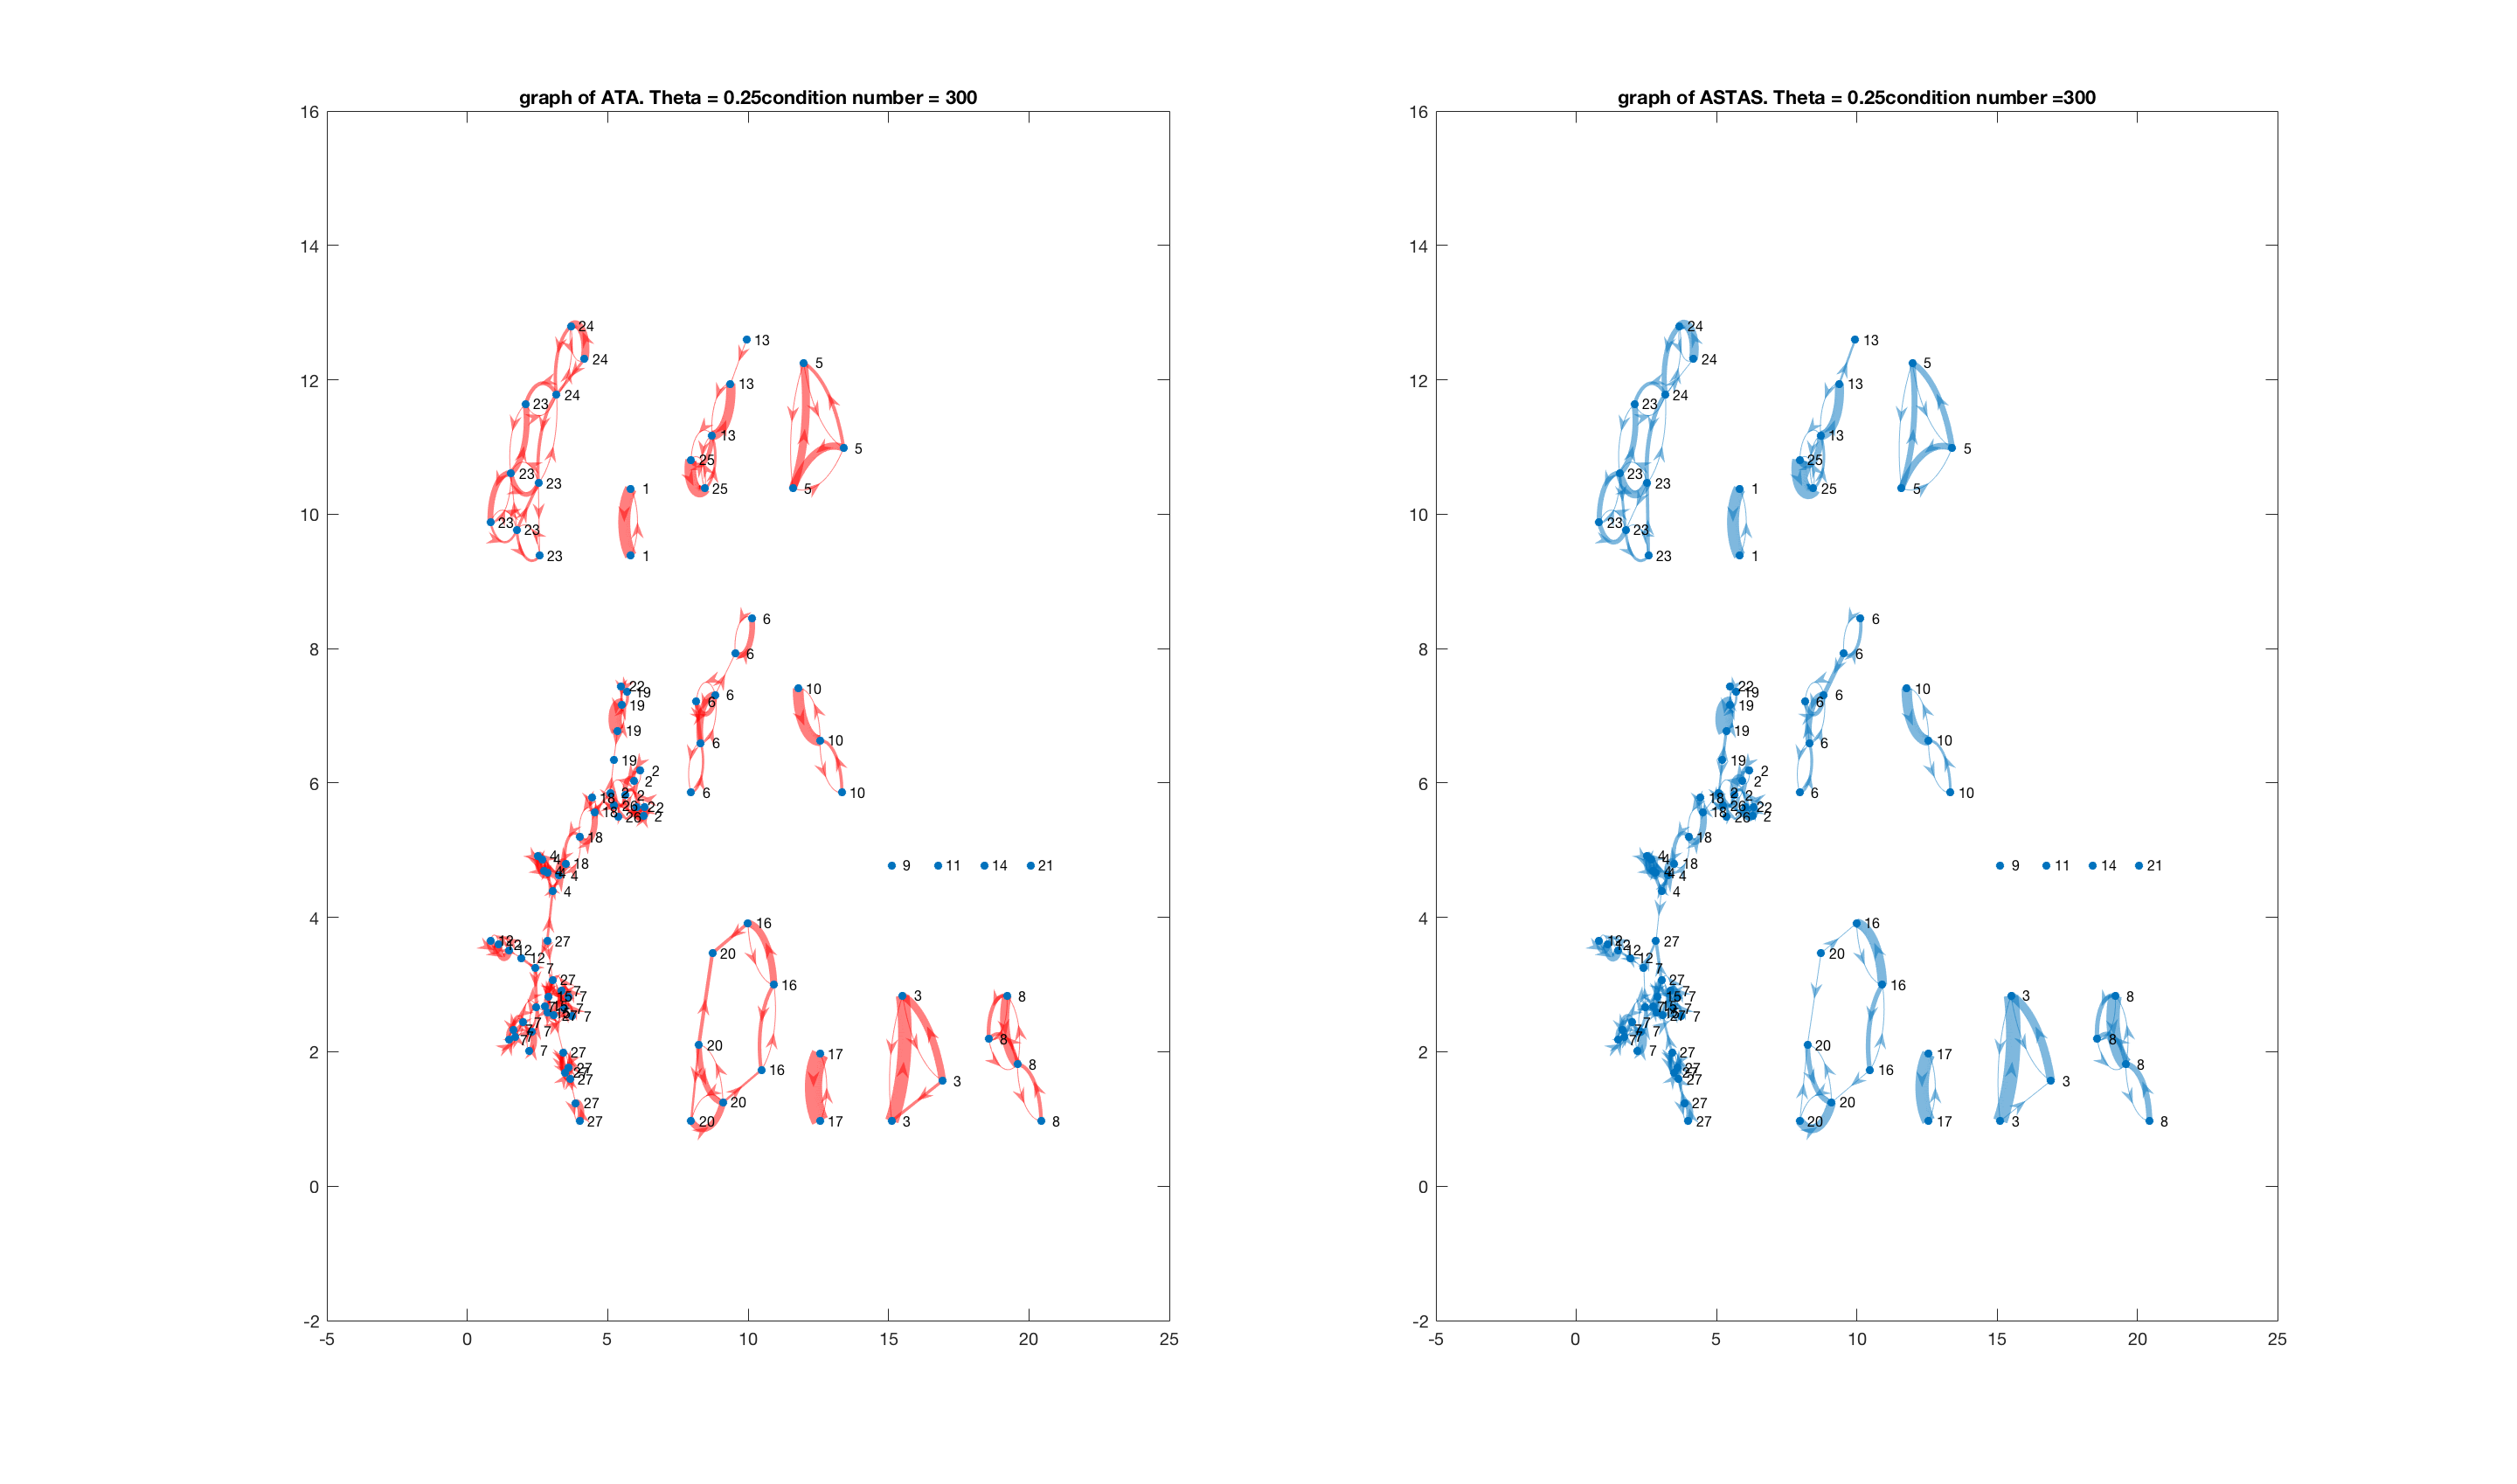
\includegraphics[width=1\textwidth]{sampling.png}
\end{figure}



%------------------------------------------------

\subsection{Performance}
%------------------------------------------------
\subsubsection{Well Conditioned Incoherent Matrix}
Performance: Well Conditioned Incoherent Matrix
The incoherent matrix (coherence $\mu(A)$ is small) is constructed by
$$
A = randn(m,n);
$$

\begin{table}\label{table_inc}
\centering
\caption{Incoherent Random Matrix}
\begin{tabular}{| l | l | l |l |l |l |l |l |l |l |}\hline
  m & n & Size  &   Conde    &    PCG.res    &  PCG.iter    &  TW.res    &  TW.iter  &   AMG.res    &  AMG.iter\\\hline
3000& 109 &  3.27e+05  & 8.0592  & 2.8265e-08  & 10  &  7.8964e-08  & 11  & 8.6322e-11 & 3   \\\hline
 5000 & 141 &7.05e+05  & 7.1294 &  6.3485e-08   & 9    & 5.0459e-08   & 11 & 6.8662e-12  & 3  \\\hline
  10000& 200 &   2e+06    & 7.6457   & 1.8065e-08   & 9    & 3.3853e-08   &11 &1.2271e-12   &3 \\\hline
   20000& 282 & 5.64e+06   &7.4708  &  3.6032e-08 &    8   &   3.4031e-08 &   11& 3.468e-13   &3  \\\hline
  40000& 400 &  1.6e+07  &  7.3094 &   8.8878e-08  &   7  &    2.8748e-08  &  11 &  3.6036e-14   & 3  \\\hline
\end{tabular}
\end{table}


%------------------------------------------------
\subsubsection{Well Conditioned Semicoherent Matrix}

Performance: Well Conditioned Semicoherent Matrix
\small
{Semicoherent matrix is given by
$$
A_{m \times n} =
 \begin{bmatrix}
  B & \\
    \quad & I_{n/2}
 \end{bmatrix},
$$
where $B$ us an $(m - n/2) \times n/2$ rectangular random matrix and $I_{n/2}$ is a square identity of dimension $n/2$. }


\begin{table}\label{table_semi}
\centering
\caption{Semicoherent Matrix with Row Sampling}
\begin{tabular}{| l | l | l |l |l |l |l |l |l |l |}\hline
  m & n & Size  &   Conde    &    PCG.res    &  PCG.iter    &  TW.res    &  TW.iter  &   AMG.res    &  AMG.iter\\\hline
3000& 109 &  3.24e+05 &  3.7979   & 4.4898e-08  &  8    &   6.2979e-08    &13    &  3.7059e-13   &  3   \\\hline
 5000 & 141 &    7e+05  & 3.6879   & 2.3175e-08 &   8     &  3.6585e-08    &12 &    5.6326e-14    & 3   \\\hline
  10000& 200 &     2e+06  &  3.7234   & 5.1245e-08  &  7   &    3.7377e-08 &   13   &   6.3799e-08   & 2    \\\hline
   20000& 282 &  5.64e+06  & 3.6137  &  2.4414e-08  &  7   &    4.0871e-08 &   12   &  3.5634e-08  &  2   \\\hline
   40000 & 400 & 1.6e+07   &  3.4741  &   8.1149e-08  &   6     &   4.6966e-08  & 12 &  1.094e-08 &   2  \\\hline
\end{tabular}
\end{table}


%------------------------------------------------
\subsubsection{Ill Conditioned Sparse Random Matrix}
Performance: Ill Conditioned Sparse Random Matrix
The sparse random matrix is generated by the MATLAB's function $sprand$
$$
 A = sprand(m,n,s,1/c);
$$
where $m$ is the number of rows, $n$ is the number of columns, $s$ is the sparsity and $c$ is the estimated condition number.
\\


%------------------------------------------------
Performance: Ill Conditioned Sparse Random Matrix

\begin{table}\label{table_spc}
\centering
\caption{Sparse Random Matrix Using Uniform Sampling $m = 40000, n = 200.$}
\begin{tabular}{|*{8}{c|}}\hline
     Nnz    &   Conde     &  PCG.res    &  PCG.iter   &   TW.res   &   TW.iter   &   AMG.res    &  AMG.iter \\\hline
    38942  &      2132.1  &  8.7014e-08   & 106    &     6.5273e-08   & 33     &    3.7773e-08  &  23   \\\hline
    38228   &      12321   & 9.6274e-08    & 167    &     7.8268e-08   & 44     &    9.9291e-08  &  36    \\\hline
    37718    &     73525    & 2.8338e-05    & 200    &     4.6732e-08   & 79     &    6.1329e-08  &  57    \\\hline
    38178     &    71728    & 2.7356e-07    & 200     &    8.5303e-08    &52      &   3.6577e-08   & 42     \\\hline
    37730    & 3.9579e+05  &    0.002827   & 121    &     6.8812e-08   & 76      &   3.2188e-08  &  58     \\\hline
\end{tabular}
\end{table}
\begin{table}
\centering
\caption{Sparse Random Matrix Using Row Sampling $m = 40000, n = 200.$}
\begin{tabular}{|*{8}{c|}}\hline
     Nnz    &   Conde    &    PCG.res    &  PCG.iter    &  TW.res    &  TW.iter  &   AMG.res    &  AMG.iter\\\hline
    38942  &      2132.1  &  8.7014e-08  &  106      &   5.3535e-08  &  30    &     3.6095e-08  &  23      \\\hline	
    38228   &      12321   & 9.6274e-08   & 167       &  9.2237e-08   & 44      &   9.9291e-08   & 36      \\\hline
    37718    &     73525   & 2.8338e-05    & 200       &  8.9378e-08   & 75      &   6.1329e-08   & 57      \\\hline
    38178     &   71728    & 2.7356e-07    & 200        & 4.0376e-08    &58       &  3.8837e-08    &42      \\\hline
    37730    & 3.9579e+05  &    0.002827  &  121      &   4.7336e-08   & 81      &   6.2102e-08   & 57  \\\hline


\end{tabular}
\end{table}

\begin{itemize}
\item The iteration steps depend weakly on the condition number $\kappa(A). $
\end{itemize}

%------------------------------------------------
\subsubsection{UDV Matrix}
Performance: UDV Matrix
UDV matrix is a random matrix generated by
$$
A = U D V,
$$
where $U$ is an $m \times n$ orthonormal matrix, $V$ is an $n \times n$ orthonormal matrix and
$D = diag[1,1+(c-1)/n,\cdots,c]$.

\begin{table}\label{}
\caption{UDV Matrix Using CoarsenAMGa and Row Sampling $m = 10000, n = 200.$}
\begin{tabular}{|*{8}{c|}}\hline
  Nnz    &   Conde  &      PCG.res   &   PCG.iter     & TW.res  &    TW.iter     &   AMG.res &     AMG.iter \\\hline
      40000  &      3468.1 &   9.1949e-08  &  112     &    9.4608e-08  &  29       & 9.9643e-08  &  25      \\\hline
    40000   &      16679  &  8.3161e-08 &   192     &    5.4534e-08   & 50           & 5.7913e-08    &43      \\\hline
    40000  & 1.0667e+05  &  3.5074e-06 &   198    &     9.0271e-08 &   73      &   7.1027e-08   & 61     \\\hline
    40000  &  4.0013e+05  &   2.199e-05  &  190     &    8.3462e-08  &  81       &  6.5267e-08   & 66     \\\hline
    40000   & 1.0203e+06  &  1.8215e-05  &  197    &     9.5749e-08   & 83        & 1.1792e-08  &  68    \\\hline
\end{tabular}
\end{table}


%------------------------------------------------

\subsubsection{Graph Laplacian Matrix}
Performance: Graph Laplacian Matrix
Given edges and generate the graph laplacian matrix $G$ by
\begin{lstlisting}
        i = repmat(1:size(edge,1),1,2)';
        i = i(:);
        j = edge(:);
        s = repmat([-1 1],size(edge,1),1);
        s = s(:);
        B = sparse(i,j,s);
        G = B'*B;
\end{lstlisting}


\begin{table}\label{}
\caption{Graph Laplacian Matrix Using CoarsenAMGc $m = 9314,n=100$}
\begin{tabular}{|*{8}{c|}}\hline
  Nnz    &   Conde  &      PCG.res   &   PCG.iter     & TW.res  &    TW.iter    &   AMG.res &     AMG.iter \\\hline
9214     &   10.273  &   4.0992e-08   & 17       &   4.4332e-08  &  12         &5.7114e-10  &   4    \\\hline
    9214  &      112.71 &   6.6875e-08  &  37    &      7.0856e-08 &   12      &   6.4333e-08&     7   \\\hline
    9214  &      1657.1 &   8.3804e-08  &  47    &       8.406e-08 &   15    &   9.248e-08  &   9     \\\hline
    9214  &       26188 &    4.0137e-08  &  51   &       8.7113e-08  &  17     &   4.2357e-08  &  10   \\\hline
    9214  &  4.1839e+05 &   6.1113e-08   & 41   &       3.2572e-08  &  19     &    3.5725e-08 &   11  \\\hline
\end{tabular}
\end{table}





%------------------------------------------------

\subsection{Convergence Analysis}
\begin{theorem}[Sum of Rank-1 Matrix]
Let $y_1,y_2,\cdots,y_n$ be i.i.d. random column vectors in $\bbbc^d$ with
$$
\| y_i \| \leq M \quad \text{and} \quad \|\E[y_i y_i^*] \| \leq 1.
$$
Then for all $0 \leq \epsilon \leq 1$
$$
Pr \left( \| \frac{1}{n} \sum_{k=1}^n y_k y_k^* - \E [y_1 y_1^T] \| \geq \epsilon \right) \leq
2d exp(-\frac{3 n \epsilon^2}{8 (M^2+1)}).
$$
\end{theorem}

%------------------------------------------------
\subsubsection{Row Sampling}
Let
$$
y_k = \begin{cases} & A_i^T/ \sqrt{p_i}  \quad \text{with probability} \quad p_i, \quad 1 \leq i \leq m;  \\
                               & 0 \quad \quad \text{otherwise}.
        \end{cases}
$$

$$
\E [y_k y_k^T] = \sum_{i=1}^m A_i^T A_i = A^T A.
$$

Randomly choose r $y_i$'s. Put them together to get the sampled matrix $As$. Then
$$
As^T As = \frac{1}{r} \sum_{i=k}^r y_k y_k^T.
$$
By the Theorem (Sum of Rank-1 Matrix)
$$
\| As^T As - A^T A \| \leq \epsilon  \quad \text{with high probability}.
$$


\subsubsection{High Frequency and Low Frequency}

With high probability, $\forall x \neq 0,$
\begin{equation}\label{star}
|(A^TA x,x) - \epsilon^2(x,x) | \leq (As^T As x,x) \leq (A^TA x,x) + \epsilon^2(x,x).
\end{equation}

For the matrix $A^T A$ after normalization, $0 < \lambda_{min} \leq \lambda_{max} \leq c$. \\
For high frequency eigenvectors, i.e.
$$
(A^T Ax,x)  \approx \lambda_{max} \|x\|^2
$$
we have
$$
(A_s^T A_s x,x) \leq c (A^TAx,x).
$$

But for low frequency eigenvectors, we need the coarsening part.






%\begin{thebibliography}{99}

%\bibitem{CON2015} Peter Oswald, Weiqi Zhou
% Convergence analysis for Kaczmarz-type methods in a Hilbert space framework
%\emph{Linear algebra and its Applications} 478(2015),131-161.

%\bibitem{FLSA2011} P. Drineas, M. W. Mahoney, S. Muthukrishnan and T. Sarlos
%\newblock Faster least squares approximation
%\newblock \emph{Numerische Mathematik} (2011) 117: 219. %doi:10.1007/s00211-010-0331-6

%\bibitem{SRFT2008} V. Rokhlin and M. Tygert
%\newblock A Fast Randomized Algorithm for Overdetermined Linear Least-Squares %Regression,
%\newblock  \emph{Proceedings of the National Academy of Science of the United States of America,}  Vpl. 105, No.36(Sep.9,2008),pp. 13212-13217


%\bibitem{BLEN2010} H. Avron, P. Maymounkov and S. Toledo
%\newblock Blendenpik: Supercharging LAPACK's Least-Squares Solver
%\newblock \emph{ SIAM Journal on Scientific Computing}
%32.3 (2010): 1217. c2010 Society for Industrial and Applied Mathematics

%\bibitem{ARK01} Ji Liu and Stephen J. Wright, An Accelerated Randomized Kaczmarz Algorithm, \emph{Mathematics of Computation}, Volume 85, Number 297, January 2016, pp. 153--178.

%\bibitem{ITE01}
%Long Chen, Classical Iterative Methods, available at
%\url{http://www.math.uci.edu/~chenlong/226/Ch6IterativeMethod.pdf}.


%\bibitem{WikiRK} ] Randomized Kaczmarz Method, available at
%\url{https://en.wikipedia.org/wiki/Kaczmarz_method}.

%\end{thebibliography}
